\documentclass[en,12pt]{latex/elegantbookr}


\hypersetup{
  pdfcreator={LaTeX via pandoc}}


\usepackage{longtable,booktabs}



\setlength{\emergencystretch}{3em}  % prevent overfull lines
\providecommand{\tightlist}{%
  \setlength{\itemsep}{0pt}\setlength{\parskip}{0pt}}

\setcounter{secnumdepth}{5}

%%% Use protect on footnotes to avoid problems with footnotes in titles
\let\rmarkdownfootnote\footnote%
\def\footnote{\protect\rmarkdownfootnote}

  \title{Algebra and Geometry of Elementary Functions}


  \author{Fei Ye}

  \date{2020-01-29}

% logo 图案
% 封面图片
% 版本号
  \version{0.01}
% 机构名
% 引用格言
% 导言区 preamble
\usepackage{framed,color}
\definecolor{shadecolor}{RGB}{248,248,248}


%%%%%%%%%%%%%%%%%%%%%%%%% Adjust words spacing %%%%%%%%%%%%%%%%%%
\usepackage[protrusion=true,expansion=true]{microtype}
%%%%%%%%%%%%%%%%%%%%%%%%%%%%%%%%%%%%%%%%%%%%%%%%%%%%%%%%%%%%%%%%%

%%%%%%%%%%%%%%%%%%% Packages for Math %%%%%%%%%%%%%%%%%%%%%%%%%%
\usepackage{mathtools}
% \usepackage{breqn}
%%%%%%%%%%%%%%%%%%%%%%%%%%%%%%%%%%%%%%%%%%%%%%%%%%%%%%%%%%%%

%%%%%%%%%%%%%%%%%%%%%%%%%% Font Encoding Packages %%%%%%%%%%%%%%%%%%%%%%%
% \usepackage[utf8]{inputenc}

% \usepackage[T1]{fontenc}  % use this if European fonts (ec) package is installed
%%%%%%%%%%%%%%%%%%%%%%%%%%%%%%%%%%%%%%%%%%%%%%%%%%%%%%%%%%%%%%%%%%%%%%%%%%%%%%

%%%%%%%%%%%%%%%%%%%%%%%%%%%%%% Font Packages %%%%%%%%%%%%%%%%%%%%%%%%%%%%%%%
% \usepackage{libertine}  %%%%%The Linux Libertine font family
% \usepackage[libertine]{newtxmath}

% \usepackage[expert,altbullet,vargreek,noamssymbols]{lucidabr}
% \usepackage[expert,vargreek,noamssymbols]{lucbmath}


% \usepackage{charter}    %%%%%%Good for screen display
% \usepackage[charter]{mathdesign}
%%%%%%%%%%%%%%%%%%%%%%%%%%%%%%%%%%%%%%%%%%%%%%%%%%%%%%%%%%%%%%%%%%%%%%%%%%%%%%%%%%%%%%%%%

\hypersetup{
	linktoc=all
}

\usepackage{color}
% \usepackage[table]{xcolor}

\definecolor{greenbean}{RGB}{144,237,204}
%\pagecolor{greenbean}
\def\gray{\color{gray}}
\def\black{\color{black}}
\def\blue{\color{blue}}
\def\red{\color{red}}
\def\green{\color{green}}
\def\yellow{\color{yellow}}
\def\cyan{\color{cyan}}
\def\brown{\color{brown}}
\def\purple{\color{purple}}
\def\olive{\color{olive}}
\def\lime{\color{lime}}
\def\darkgray{\color{darkgray}}

%%%%%%%%%%%%%%%% Include Graphs %%%%%%%%%%%%%%%%%%%%%%
\usepackage{float}
\textfloatsep=0pt
\dblfloatsep=0pt
%%%%%%%%%%%%%%%%%%%%%%%%%%%%%%%%%%%%%%%%%%%%%%%%%%%%%%

%%%%%%%%%%%%%% Spacing for Baseline and Parskip  %%%%%%%%%%%%%%
\renewcommand{\baselinestretch}{1.1}
%%%%%%%%%%%%%%%%%%%%%%%%%%%%%%%%%%%%%%%%%%%%%%%%%%%%%%%%%%%%%%%

%%%%%% Packages for Fine Tune Content %%%%%%%%%%%
\usepackage[english]{babel}
\usepackage{indentfirst,bm}
%%%%%%%%%%%%%%%%%%%%%%%%%%%%%%%%%%%%%%%%%%%%%%%%%

%%%%%%%%%%%%%%%%%%%%%%%%%%%%%%%%%%%%%%%%%%%%%%%%%
% \usepackage{hhline}
%%%%%%%%%%%%%%%%%%%%%%%%%%%%%%%%%%%%%%%%%%%%%%%%%%%

%%%%%%%%%%%%%%%%%%%%%%%%%%%%%%%%%%%%%%%%%%%%%%%%%%%%%%%%%

%%%%%%%%%%add blank pages%%%%%%%%%
% \usepackage{afterpage}
\newcommand\blankpage{%
\null
    \thispagestyle{empty}%
    % \addtocounter{page}{-1}%
    \newpage
}
%%%%%%%%%%%%%%%%%%%%%%%%%%%%%%%%%%%%%%%%%%%%%%%%%%%%%%


%%%%%%%%%%%%%%%%%% Enumerate Style %%%%%%%%%%%%%%%%%%%%%%%%%%
\usepackage[inline]{enumitem}
\setenumerate{
	% label=\textup{(\arabic*)},
	% afterlabel={\quad},
	%%vertical
	topsep=0pt,
	partopsep=0pt,
	itemsep=2pt,
	parsep=0pt,
	% labelindent=0em,
	% itemindent = *,
	itemindent=1ex,
	wide,
	itemjoin={\hspace{\fill}},
	%%Horizontal
}
\setitemize{
	%%vertical
	topsep=0pt,
	partopsep=0pt,
	itemsep=0pt,
	parsep=0pt,
	%%Horizontal
	labelindent=0em,
	leftmargin =!,
	itemindent = 0pt,
	labelsep= 2pt,
	labelwidth=1em,
}
\setlist{topsep=0pt}
%%%%%%%%%%%%%%%%%%%%%%%%%%%%%%%%%%%%%%%%%%%%%%%%%%%%%%%%%

%%%%%%%%%%%%% Remove Vertical Some Spacing%%%%%%%%%%%%%%%
\makeatletter
\def\example@space@setup{
	\example@preskip=2pt
	\example@postskip=0
}
\makeatother

% \makeatletter
% \def\exercise@space@setup{%
%   \exercise@preskip=0 \exercise@postskip=\exercise@preskip
% }
% \makeatother

\makeatletter
\def\solution@space@setup{
	\solution@preskip=-\medskip
	\solution@postskip=0
}
\makeatother

% \makeatletter
% \def\proof@space@setup{
% 	\proof@preskip=0pt
% 	\proof@postskip=0pt
% }
% \makeatother

%%%%%%%%%%%%%%%%%%%%%%%%%%%%%%%%%%%%%%%%%%%%%%%%%%%%%%%%%%%%%%%%%

%%%%%%%%%%%% Packages for Pictures and Commutative Diagrams%%%%%%
\usepackage{tikz}
\usepackage{pgfplots}
\pgfplotsset{compat=newest}
\usepackage{pgfmath}
\usepackage{tikz-cd}
\usepackage{pgffor}
\usepackage{tkz-euclide}
\usetkzobj{all}
\usepgfplotslibrary{fillbetween}
\usetikzlibrary{
	calc,
	angles,
	quotes,
	arrows.meta,
	decorations.markings,
	math,
	backgrounds,
	pgfplots.statistics,
	matrix,
	patterns,
	shapes.geometric,
	spy,
	intersections,
}
%%%%%%%%%%%%%%%%%%%%%%%%%%%%%%%%%%%%%%%%%%%%%%%%%%%%%%%%%%%%%%%%%%%%

%%%%%%%%%%%%%%%%% Setup the Coordinate System %%%%%%%%%%%%%%%%%%%%%%
\pgfplotsset{every axis/.style={
			%		 axis equal image,
			axis x line=middle,    % put the x axis in the middle
			axis y line=middle,    % put the y axis in the middle
			axis line style={-latex,very thick}, % arrows on the axis
			xlabel={$x$},          % default put x on x-axis
			ylabel={$y$},          % default put y on y-axis
			xlabel style = {font=\tiny, at={(xticklabel* cs:1)}, anchor=south},
			ylabel style = {font=\tiny, at={(yticklabel* cs:1)}, anchor=west},
			scaled ticks=true,
			x tick label style={font=\tiny, yshift=0.25ex, inner xsep=0pt},
			y tick label style={font=\tiny, xshift=0.25ex, inner ysep=0pt},
			grid style={black},
			% set layers=standard,
		}
}

%%%%%%%%%%%%%%% include files/Figure %%%%%%%%%%%%%%%%%%%%%%%%%%%%%%%%%
% \usepackage{import}
% \usepackage{subfiles}
\usepackage[verbose]{wrapfig}
%%%%%%%%%%%%%%%%%%%%%%%%%%%%%%%%%%%%%%%%%%%%%%%%%%%%%%%%%%%%%%%%%

%%%%%%%%%%%%%%%% Cancel common factors in Math %%%%%%%%%%%%%%%%%%%%
\usepackage[makeroom]{cancel}
%%%%%%%%%%%%%%%%%%%%%%%%%%%%%%%%%%%%%%%%%%%%%%%%%%%%%%%%%%%%%%%%%%%

%%%%%%%%%%%%%% Math mode without vertical spacing %%%%%%%%%%%%%%%%%
\makeatletter
\g@addto@macro\normalsize{%
	\setlength\abovedisplayskip{1pt plus 2pt minus 2pt}%
	\setlength\belowdisplayskip{1pt plus 2pt minus 2pt}%
	\setlength\abovedisplayshortskip{1pt plus 2pt minus 2pt}%
	\setlength\belowdisplayshortskip{1pt plus 2pt minus 2pt}%
}
\makeatother
%%%%%%%%%%%%%%%%%%%%%%%%%%%%%%%%%%%%%%%%%%%%%%%%%%%%%%%%%%%%%%%%


%%%%%%%%%%%%%%%%%%%%%
%%% Redefine the original definition of \paragraph in the article
\makeatletter
\renewcommand{\paragraph}{%
  \@startsection{paragraph}{4}%
  {\z@}{1ex \@plus 0.2ex \@minus .2ex}{-1ex}%
  {\normalfont\large\bfseries}%
}
\makeatother

\addto\captionsenglish{%
	\renewcommand{\chaptername}{Lesson \thechapter}
}

\newcommand{\ZZ}{\mathbf{Z}}
\newcommand{\RR}{\mathbf{R}}
\newcommand{\NN}{\mathbf{N}}
\newcommand{\QQ}{\mathbf{Q}}
\newcommand{\abs}[1]{\lvert #1\rvert}
\newcommand{\ii}{\mathbf{i}}
\newcommand{\parll}{ {\mathbin{\parallel}} }
\newcommand{\prll}{{\mathbin{\!/\mkern-5mu/\!}}}

\makeatletter
\newcommand*\rel@kern[1]{\kern#1\dimexpr\macc@kerna}
\newcommand*\widebar[1]{%
\begingroup
\def\mathaccent##1##2{%
\rel@kern{0.8}%
\overline{\rel@kern{-0.8}\macc@nucleus\rel@kern{0.2}}%
\rel@kern{-0.2}%
}%
\macc@depth\@ne
\let\math@bgroup\@empty \let\math@egroup\macc@set@skewchar
\mathsurround\z@ \frozen@everymath{\mathgroup\macc@group\relax}%
\macc@set@skewchar\relax
\let\mathaccentV\macc@nested@a
\macc@nested@a\relax111{#1}%
\endgroup
}
\renewcommand{\bar}{\widebar}
\newcommand*\centermath[1]{\omit\hfil~$\displaystyle#1$~\hfil\ignorespaces}
\newcommand{\cmc}{\centermath}
\newcommand*\ctc[1]{\omit\hfil\quad~ #1 ~\quad\hfil\ignorespaces}
\newcommand{\dfn}[1]{\textit{\textbf{#1}}}


\newlength{\lengthsignature}
\settowidth{\lengthsignature}{Summer 2018}

\usepackage{longtable}

\geometry{
	letterpaper,
	top=0.9in,
	bottom=0.8in,
	left=0.8in,
	right=0.8in,
	% footsep=0pt
	}

\usepackage[export]{adjustbox}

% \fancyheadoffset[LO,LE]{0cm}

% \fancyfoot[L]{\raisebox{-0.6\baselineskip}{
\includegraphics[height=1.2\baselineskip, valign=c]{pics/by-nc-sa.eps}}}

% \fancyfoot[R]{\raisebox{-0.6\baselineskip}{\hfill \scriptsize \sffamily A Concise Workbook for College Algebra}\hspace{-1ex}}


\setlength\columnsep{10pt}
\setlength{\footskip}{6pt}
\setlength{\parindent}{0pt}
\setlength{\parskip}{0pt plus 1pt minus 1pt}
\setlength{\parsep}{2pt plus 1pt minus 1pt}
\setlength{\topsep}{2pt plus 1pt minus 1pt}
\setlength{\multicolsep}{1pt plus 1pt minus 1pt}

\def\rotationdegree{180}

\raggedcolumns % to align multicols by top.


\frontmatter

\usepackage{amsthm}
\newtheorem{theorem}{Theorem}[chapter]
\newtheorem{lemma}{Lemma}[chapter]
\newtheorem{corollary}{Corollary}[chapter]
\newtheorem{proposition}{Proposition}[chapter]
\newtheorem{conjecture}{Conjecture}[chapter]
\theoremstyle{definition}
\newtheorem{definition}{Definition}[chapter]
\theoremstyle{definition}
\newtheorem{example}{Example}[chapter]
\theoremstyle{definition}
\newtheorem{exercise}{Problem}[chapter]
\theoremstyle{remark}
\newtheorem*{remark}{Remark}
\newtheorem*{solution}{Solution}
\let\BeginKnitrBlock\begin \let\EndKnitrBlock\end
\begin{document}
% 封面
\maketitle
% 插入 before_body.tex

% 目录
{
\setcounter{tocdepth}{1}
\tableofcontents
}
% 表目录
% 图目录
% 书籍主体部分
\hypertarget{introduction}{%
\chapter*{Introduction}\label{introduction}}
\addcontentsline{toc}{chapter}{Introduction}

This notebook is intended to give a brief introduction to elementary functions emphasizing on effective thinking in algebra and geometry.

In the first part, we will review mathematical operations including addition, multiplication, \(n\)-th root, exponentiation and logarithm.

In the second part, we will study the concepts of functions, algebraic functions and their applications.

In the third part, we will study elementary transcendental functions and applications.

Comments and suggestions are very welcome.

This work is licensed under a \href{https://creativecommons.org/licenses/by-nc-sa/4.0/}{Creative Commons Attribution-NonCommercial-ShareAlike 4.0 International License}.

\begin{figure}
\centering

\includegraphics{figs/by-nc-sa.png}
\caption{by-nc-sa license icon}
\end{figure}

\hypertarget{part-part-i-mathematical-operations}{%
\part*{Part I: Mathematical Operations}\label{part-part-i-mathematical-operations}}
\addcontentsline{toc}{part}{Part I: Mathematical Operations}

\hypertarget{integer-exponents}{%
\chapter{Integer Exponents}\label{integer-exponents}}

\hypertarget{dont-be-tricked}{%
\section{Don't Be Tricked}\label{dont-be-tricked}}

\BeginKnitrBlock{rmdthink}
A pizza shop sales 12-inches pizza and 8-inches pizza at the price \$12/each and \$6/each respectively. With \$12, would you like to order one 12-inches and two 8-inches. Why?
\EndKnitrBlock{rmdthink}

\BeginKnitrBlock{rmdthink}
A sheet of everyday copy paper is about 0.01 millimeter thick. Repeat folding along a different side 20 times. Now, how thick do you think the folded paper is?
\EndKnitrBlock{rmdthink}

\hypertarget{properties-of-exponents}{%
\section{Properties of Exponents}\label{properties-of-exponents}}

For an integer \(n\), and an expression \(x\), the mathematical operation of the \(n\)-times repeated multiplication of \(x\) is call exponentiation, written as \(x^n\), that is,
\[
x^n=\underbrace{x\cdot x \cdots x}_{n \text{factors of} x}.
\]

In the notation \(x^n\), \(n\) is called \textbf{\emph{the exponent}}, \(x\) is called \textbf{\emph{the base}}, and \(x^n\) is called \textbf{\emph{the power}}, read as ``\(x\) raised to the \(n\)-th power'', ``\(x\) to the \(n\)-th power'', ``\(x\) to the \(n\)-th'', ``\(x\) to the power of \(n\)'' or ``\(x\) to the \(n\)''.

\begin{longtable}[]{@{}ll@{}}
\toprule
\begin{minipage}[b]{0.47\columnwidth}\raggedright
Property\strut
\end{minipage} & \begin{minipage}[b]{0.47\columnwidth}\raggedright
Example\strut
\end{minipage}\tabularnewline
\midrule
\endhead
\begin{minipage}[t]{0.47\columnwidth}\raggedright
The product rule \[x^m\cdot x^n=x^{m+n}.\]\strut
\end{minipage} & \begin{minipage}[t]{0.47\columnwidth}\raggedright
\[2x^2\cdot (-3x^3)=-6x^5.\]\strut
\end{minipage}\tabularnewline
\begin{minipage}[t]{0.47\columnwidth}\raggedright
The quotient rule (for \(x\neq 0\).) \[\dfrac{x^m}{x^n}= \begin{cases} x^{m-n}  & \text{if} m\ge n.\\[1em] \dfrac{1}{x^{n-m}} & \text{if} m\le n. \end{cases} \]\strut
\end{minipage} & \begin{minipage}[t]{0.47\columnwidth}\raggedright
\[\frac{15x^5}{5x^2}=3x^3;\] \[\frac{-3x^2}{6x^3}=-\frac{1}{2x}.\]\strut
\end{minipage}\tabularnewline
\begin{minipage}[t]{0.47\columnwidth}\raggedright
The zero exponent rule (for \(x\neq 0\).) \[x^0=1.\]\strut
\end{minipage} & \begin{minipage}[t]{0.47\columnwidth}\raggedright
\[(-2)^0=1;\] \[-x^0=-1.\]\strut
\end{minipage}\tabularnewline
\begin{minipage}[t]{0.47\columnwidth}\raggedright
The negative exponent rule (for \(x\neq 0\).) \[x^{-n}=\dfrac{1}{x^n} \quad\text{and}\quad \dfrac{1}{x^{-n}}=x^n.\]\strut
\end{minipage} & \begin{minipage}[t]{0.47\columnwidth}\raggedright
\[(-2)^{-3}=\frac{1}{(-2)^3}=-\frac18;\] \[\frac{x^{-2}}{x^{-3}}=\frac{x^3}{x^2}=x.\]\strut
\end{minipage}\tabularnewline
\begin{minipage}[t]{0.47\columnwidth}\raggedright
The power to a power rule \[\left(x^a\right)^b=x^{ab}.\]\strut
\end{minipage} & \begin{minipage}[t]{0.47\columnwidth}\raggedright
\[\left(2^{2}\right)^3=2^6=64;\] \[\left(x^2\right)^3=x^6.\]\strut
\end{minipage}\tabularnewline
\begin{minipage}[t]{0.47\columnwidth}\raggedright
The product raised to a power rule \[(xy)^n=x^ny^n.\]\strut
\end{minipage} & \begin{minipage}[t]{0.47\columnwidth}\raggedright
\[\left(-2x\right)^{2}=(-2)^2x^2=4x^2.\]\strut
\end{minipage}\tabularnewline
\begin{minipage}[t]{0.47\columnwidth}\raggedright
The quotient raised to a power rule (for \(y\neq 0\).) \[\left(\dfrac{x}{y}\right)^n=\dfrac{x^n}{y^n}.\]\strut
\end{minipage} & \begin{minipage}[t]{0.47\columnwidth}\raggedright
\[    \left(\dfrac{x}{-2}\right)^{3}=\dfrac{x^3}{(-2)^3}=-\dfrac{x^3}{8}.\]\strut
\end{minipage}\tabularnewline
\bottomrule
\end{longtable}

\BeginKnitrBlock{rmdnote}
\textbf{Order of Basic Mathematical Operations}

In mathematics, the order of operations reflects conventions about which procedure should be performed first. There are four levels (from the highest to the lowest):

\textbf{Parenthesis}; \textbf{Exponentiation}; \textbf{Multiplication and Division}; \textbf{Addition and Subtraction}.

Within the same level, the convention is to perform from the left to the right.
\EndKnitrBlock{rmdnote}

\hypertarget{examples}{%
\section{Examples}\label{examples}}

\BeginKnitrBlock{example}
\protect\hypertarget{exm:unnamed-chunk-4}{}{\label{exm:unnamed-chunk-4} }
Simplify. \textbf{Write with positive exponents.}
\[
\left(\dfrac{2y^{-2}z^{-5}}{4x^{-3}y^6}\right)^{-4}.
\]
\EndKnitrBlock{example}

\BeginKnitrBlock{solution}
\iffalse{} {Solution. } \fi{}
\[
\left(\dfrac{2y^{-2}z^{-5}}{4x^{-3}y^6}\right)^{-4}
=\left(\dfrac{x^3}{2z^{5}y^8}\right)^{-4}
=\left(\dfrac{2z^{5}y^8}{x^3}\right)^4
=\dfrac{2^4(z^{5})^4(y^8)^4}{(x^3)^4}
=\dfrac{16y^{32}z^{20}}{x^{12}}.
\]
\EndKnitrBlock{solution}

\BeginKnitrBlock{rmdtip}
\textbf{Simplify (at least partially) the problem first}

To avoid mistakes when working with negative exponents, it's better to apply the negative exponent rule to change negative exponents to positive exponents and simplify the base first.
\EndKnitrBlock{rmdtip}

\hypertarget{practice}{%
\section{Practice}\label{practice}}

\BeginKnitrBlock{exercise}
\protect\hypertarget{exr:unnamed-chunk-7}{}{\label{exr:unnamed-chunk-7} }
Simplify. \textbf{Write with positive exponents.}

\begin{enumerate}
\def\labelenumi{\arabic{enumi}.}
\tightlist
\item
  \((3a^2b^3c^2)(4abc^2)(2b^2c^3)\)
\item
  \(\dfrac{4y^3z^0}{x^2y^2}\)
\item
  \((-2)^{-3}\)
\end{enumerate}
\EndKnitrBlock{exercise}

\BeginKnitrBlock{exercise}
\protect\hypertarget{exr:unnamed-chunk-8}{}{\label{exr:unnamed-chunk-8} }
Simplify. \textbf{Write with positive exponents.}

\begin{enumerate}
\def\labelenumi{\arabic{enumi}.}
\tightlist
\item
  \(\dfrac{-u^0v^{15}}{v^{16}}\)
\item
  \((-2a^3b^2c^0)^3\)
\item
  \(\dfrac{m^5 n^{2}}{(mn)^3}\)
\end{enumerate}
\EndKnitrBlock{exercise}

\BeginKnitrBlock{exercise}
\protect\hypertarget{exr:unnamed-chunk-9}{}{\label{exr:unnamed-chunk-9} }
Simplify. \textbf{Write with positive exponents.}

\begin{enumerate}
\def\labelenumi{\arabic{enumi}.}
\tightlist
\item
  \((-3a^2x^3)^{-2}\)
\item
  \(\left(\dfrac{-x^0y^3}{2wz^2}\right)^3\)
\item
  \(\dfrac{3^{-2}a^{-3}b^5}{x^{-3}y^{-4}}\)
\end{enumerate}
\EndKnitrBlock{exercise}

\BeginKnitrBlock{exercise}
\protect\hypertarget{exr:unnamed-chunk-10}{}{\label{exr:unnamed-chunk-10} }
Simplify. \textbf{Write with positive exponents.}

\begin{enumerate}
\def\labelenumi{\arabic{enumi}.}
\tightlist
\item
  \(\left(-x^{-1}(-y)^2\right)^3\)
\item
  \(\left(\dfrac{6x^{-2}y^5}{2y^{-3}z^{-11}}\right)^{-3}\)
\item
  \(\dfrac{(3 x^{2} y^{-1})^{-3}(2 x^{-3} y^{2})^{-1}}{(x^{6} y^{-5})^{-2}}\)
\end{enumerate}
\EndKnitrBlock{exercise}

\BeginKnitrBlock{exercise}
\protect\hypertarget{exr:unnamed-chunk-11}{}{\label{exr:unnamed-chunk-11} }
A store has large size and small size watermelons. A large one cost \$4 and a small one \$1. Putting on the same table, a smaller watermelons has only half the height of the larger one. Given \$4, will you buy a large watermelon or 4 smaller ones? Why?
\EndKnitrBlock{exercise}

\hypertarget{review-of-factoring}{%
\chapter{Review of Factoring}\label{review-of-factoring}}

\hypertarget{can-you-beat-a-calculator}{%
\section{Can You Beat a Calculator}\label{can-you-beat-a-calculator}}

\BeginKnitrBlock{rmdthink}
Do you know a faster way to find the values?

\begin{enumerate}
\def\labelenumi{\arabic{enumi}.}
\item
  Find the value of the polynomial \(2x^3-98x\) when \(x=-7\).
\item
  Find the value of the polynomial \(x^2-9x-22\) when \(x=11\).
\item
  Find the value of the polynomial \(x^3-2x^2-9x+18\) when \(x=-3\).
\item
  Find the value of \(16^2-14^2\).
\end{enumerate}
\EndKnitrBlock{rmdthink}

\hypertarget{factor-by-removing-the-gcf}{%
\section{Factor by Removing the GCF}\label{factor-by-removing-the-gcf}}

\textbf{\emph{The greatest common factor (GCF)}} of two terms is a polynomial with the \textbf{greatest coefficient} and of the \textbf{highest possible degree} that divides each term.

To \textbf{\emph{factor a polynomial}} is to \textbf{express the polynomial as a product} of polynomials of lower degrees. The first and the easiest step is to factor out the GCF of all terms.

\BeginKnitrBlock{example}
\protect\hypertarget{exm:unnamed-chunk-13}{}{\label{exm:unnamed-chunk-13} }
Factor \(4x^3y-8x^2y^2+12x^3y^3\).
\EndKnitrBlock{example}

\BeginKnitrBlock{solution}
\iffalse{} {Solution. } \fi{}
1. Find the GCF of all terms.\\
The GCF of \(4x^3y\), \(-8x^2y^2\) and \(12x^4y^3\) is \(4x^2y\).

\begin{enumerate}
\def\labelenumi{\arabic{enumi}.}
\setcounter{enumi}{1}
\item
  Write each term as the product of the GCF and the remaining factor.\\
  \(4x^3y=(4x^2y)\cdot x\), \(-8x^2y^2=(4x^2y)\cdot (-2y)\), and \(12x^4y^3=(4x^2y)(3xy^2)\).
\item
  Factor out the GCF from each term.\\
  \(4x^3y-8x^2y^2+12x^3y^3=4x^2y\cdot(x-2y+3xy^2)\).
\end{enumerate}
\EndKnitrBlock{solution}

\hypertarget{factor-by-grouping}{%
\section{Factor by Grouping}\label{factor-by-grouping}}

For a four-term polynomial, in general, we will group them into two groups and factor out the GCF for each group and then factor further.

\BeginKnitrBlock{example}
\protect\hypertarget{exm:unnamed-chunk-15}{}{\label{exm:unnamed-chunk-15} }
Factor \(2x^2-6xy+xz-3yz\).
\EndKnitrBlock{example}

\BeginKnitrBlock{solution}
\iffalse{} {Solution. } \fi{}
1. Group the first two terms and the last two terms.
\[
    \begin{aligned}
    &2x^2-6xy+xz-3yz\\
    =&(2x^2-6xy)+(xz-3yz)
    \end{aligned}
   \]

\begin{enumerate}
\def\labelenumi{\arabic{enumi}.}
\setcounter{enumi}{1}
\item
  Factor out the GCF from each group.\\
  \[
   \begin{aligned}
   =&2x(x-3y)+z(x-3y)
   \end{aligned}
  \]
\item
  Factor out the binomial GCF.
  \[
  \begin{aligned}
  =&(x-3y)(2x+z).
  \end{aligned}
  \]
\end{enumerate}
\EndKnitrBlock{solution}

\BeginKnitrBlock{example}
\protect\hypertarget{exm:unnamed-chunk-17}{}{\label{exm:unnamed-chunk-17} }
Factor \(ax+4b-2a-2bx\).
\EndKnitrBlock{example}

\BeginKnitrBlock{solution}
\iffalse{} {Solution. } \fi{}
1. Group the first term with the third term and group the second term with the last term.
\[
\begin{aligned}
&ax+4b-2a-2bx\\
=&(ax-2a)+(-2bx+4b)
\end{aligned}
\]

\begin{enumerate}
\def\labelenumi{\arabic{enumi}.}
\setcounter{enumi}{1}
\item
  Factor out the GCF from each group.
  \[
  \begin{aligned}
  =&a(x-2)+(-2b)(x-2)
  \end{aligned}
  \]
\item
  Factor out the binomial GCF.
  \[
  \begin{aligned}
  =&(x-2)(a-2b).
  \end{aligned}
  \]
\end{enumerate}
\EndKnitrBlock{solution}

\BeginKnitrBlock{rmdtip}
\textbf{Guess and check.}\\
Once you factored one group, you may expect that the other group has the same binomial factor so that factoring may be continued.
\EndKnitrBlock{rmdtip}

\hypertarget{factor-difference-of-powers}{%
\section{Factor Difference of Powers}\label{factor-difference-of-powers}}

Factoring is closely related to solving polynomial equations. If a polynomial equation \(p(x)=0\) has a solution \(r\), then \(p(x)\) has a factor \(x-r\). For example, \(x^n-r^n=0\) has a solution \(x=r\). So the difference \(x^n-r^n\) has a factor \((x-r)\). Using long division or by induction, we obtain the following equality.

\textbf{Difference of \(n\)-th powers}

\[a^n-b^n=(a-b)(a^{n-1}+a^{n-2}b+\cdots +ab^{n-2}+b^{n-1})\]

In particular,

\[a^2-b^2=(a-b)(a+b).\]

\BeginKnitrBlock{example}
\protect\hypertarget{exm:unnamed-chunk-20}{}{\label{exm:unnamed-chunk-20} }
Factor \(25x^2-16\).
\EndKnitrBlock{example}

\BeginKnitrBlock{solution}
\iffalse{} {Solution. } \fi{}
1. Recognize the binomial as a difference of squares.
\[\begin{aligned}
&25x^2-16\\
=&(5x)^2-4^2
\end{aligned}
\]

\begin{enumerate}
\def\labelenumi{\arabic{enumi}.}
\setcounter{enumi}{1}
\tightlist
\item
  Apply the formula.
  \[
  \begin{aligned}
  =&(5x-4)(5x+4).
  \end{aligned}
  \]
\end{enumerate}
\EndKnitrBlock{solution}

\BeginKnitrBlock{example}
\protect\hypertarget{exm:unnamed-chunk-22}{}{\label{exm:unnamed-chunk-22} }
Factor \(32x^3y-2xy^5\) completely.
\EndKnitrBlock{example}

\BeginKnitrBlock{solution}
\iffalse{} {Solution. } \fi{}
\[
32x^3y-2xy^3=2xy(16x^2-y^4)=2xy((4x)^2-(y^2)^2)=2xy(4x+y^2)(4x-y^2).
\]
\EndKnitrBlock{solution}

\hypertarget{factor-trinomials}{%
\section{Factor Trinomials}\label{factor-trinomials}}

If a trinomial \(ax^2+bx+c\), \(A\neq 0\), can be factored, then it can be expressed as a product of two binomials:
\[ax^2+bx+c=(mx+n)(px+q).\]
By simplify the product using the FOIL method and comparing coefficients, we observe that
\[
a=\underbrace{mn}_{\mathrm{F}}\quad\quad\quad
b=\underbrace{mq}_{\mathrm{O}}~\underset{+}{\underset{}{+}}~\underbrace{np}_{\mathrm{I}}
\quad\quad\quad 
c=\underbrace{nq}_{\mathrm{F}}
\]

A trinomial \(ax^2+bx+c\) is also called a \textbf{\emph{quadratic polynomial}}. The function defined by \(f(x)=ax^2+bx+c\) is called a \textbf{\emph{quadratic function}}.

\BeginKnitrBlock{rmdtip}
\textbf{Trial and error.}\\
The observation suggests to use trial and error to find the undetermined coefficients \(m\), \(n\), \(p\), and \(q\) from factors of \(a\) and \(c\) such that the sum of cross products \(mq+np\) is \(b\). A diagram as shown in the following examples will be helpful to check a trial.
\EndKnitrBlock{rmdtip}

\BeginKnitrBlock{example}
\protect\hypertarget{exm:unnamed-chunk-25}{}{\label{exm:unnamed-chunk-25} }
Factor \(x^2+6x+8\).
\EndKnitrBlock{example}

\BeginKnitrBlock{solution}
\iffalse{} {Solution. } \fi{}
1. Factor \(a=1\):
\[1=1\cdot 1.\]

\begin{enumerate}
\def\labelenumi{\arabic{enumi}.}
\setcounter{enumi}{1}
\item
  Factor \(c=8\):
  \[8=1\cdot 8=2\cdot 4.\]
\item
  Choose a proper combination of pairs of factors and check if the sum of cross product equals \(b=6\):
  \[1\cdot 4+ 1\cdot 2=6.\]\\
  This step can be checked easily using the following diagram.\\
  \includegraphics[width=0.6\textwidth,height=\textheight]{figs/tikz-factoring-x\^{}2+6x+8.png}
\item
  Factor the trinomial
  \[x^2+6x+8=(x+2)(x+4).\]
\end{enumerate}
\EndKnitrBlock{solution}

\BeginKnitrBlock{example}
\protect\hypertarget{exm:unnamed-chunk-27}{}{\label{exm:unnamed-chunk-27} }
Factor \(2x^2+5x-3\).
\EndKnitrBlock{example}

\BeginKnitrBlock{solution}
\iffalse{} {Solution. } \fi{}
1. Factor \(a=2\):
\[1=1\cdot 2.\]

\begin{enumerate}
\def\labelenumi{\arabic{enumi}.}
\setcounter{enumi}{1}
\item
  Factor \(c=-3\):
  \[-3=1\cdot (-3)=(-1)\cdot 3.\]
\item
  Choose a proper combination of pairs of factors and if the sum of cross products equals \(b=5\):\\
  \[2\cdot 3+1\cdot(-1)=5.\]\\
  This step can be checked easily using the following diagram.\\
  \includegraphics[width=0.6\textwidth,height=\textheight]{figs/tikz-factoring-2x\^{}2+5x-3.png}
\item
  Factor the trinomial
  \[2x^2+5x-3=(x+3)(2x-1).\]
\end{enumerate}
\EndKnitrBlock{solution}

\BeginKnitrBlock{rmdtip}
\textbf{Use Auxiliary Problem.}\\
Some higher degree polynomials may be rewrite as a trinomial after a substitution. Factoring the trinomial helps factor the polynomial.
\EndKnitrBlock{rmdtip}

\BeginKnitrBlock{example}
\protect\hypertarget{exm:unnamed-chunk-30}{}{\label{exm:unnamed-chunk-30} }
Factor the trinomial completely.

\[4x^4-x^2-3\]
\EndKnitrBlock{example}

\BeginKnitrBlock{solution}
\iffalse{} {Solution. } \fi{}
1. Let \(x^2=y\). Then \(4x^4-x^2-3=4y^2-y-3\).

\begin{enumerate}
\def\labelenumi{\arabic{enumi}.}
\setcounter{enumi}{1}
\item
  Factor the trinomial in \(y\): \(4y^2-y-3=(4y+3)(y-1)\).
\item
  Replace \(y\) by \(x^2\) and factor further.
  \[
   \begin{split}
       4x^4-x^2-3&=4y^2-y-3\\
       &=(4y+3)(y-1)\\
       &=(4x^2+3)(x^2-1)\\
       &=(4x^2+3)(x-1)(x+1).
   \end{split}
  \]
\end{enumerate}
\EndKnitrBlock{solution}

\hypertarget{practice-1}{%
\section{Practice}\label{practice-1}}

\BeginKnitrBlock{exercise}
\protect\hypertarget{exr:unnamed-chunk-32}{}{\label{exr:unnamed-chunk-32} }
Factor out the GCF.

\begin{enumerate}
\def\labelenumi{\arabic{enumi}.}
\tightlist
\item
  \(18x^2y^2-12xy^3-6x^3y^4\)
\item
  \(5x(x-7)+3y(x-7)\)
\item
  \(-2a^2(x+y)+3a(x+y)\)
\end{enumerate}
\EndKnitrBlock{exercise}

\BeginKnitrBlock{exercise}
\protect\hypertarget{exr:unnamed-chunk-33}{}{\label{exr:unnamed-chunk-33} }
Factor by grouping.

\begin{enumerate}
\def\labelenumi{\arabic{enumi}.}
\tightlist
\item
  \(12xy-10y+18x-15\)
\item
  \(12ac-18bc-10ad+15bd\)
\item
  \(5ax-4bx-5ay+4by\)
\end{enumerate}
\EndKnitrBlock{exercise}

\BeginKnitrBlock{exercise}
\protect\hypertarget{exr:unnamed-chunk-34}{}{\label{exr:unnamed-chunk-34} }
Factor completely.

\begin{enumerate}
\def\labelenumi{\arabic{enumi}.}
\tightlist
\item
  \(25x^2-4\)
\item
  \(8x^3-2x\)
\item
  \(25xy^2+x\)
\end{enumerate}
\EndKnitrBlock{exercise}

\BeginKnitrBlock{exercise}
\protect\hypertarget{exr:unnamed-chunk-35}{}{\label{exr:unnamed-chunk-35} }
Factor completely.

\begin{enumerate}
\def\labelenumi{\arabic{enumi}.}
\tightlist
\item
  \(3x^3+6x^2-12x-24\)
\item
  \(x^4+3x^3-4x^2-12x\)
\end{enumerate}
\EndKnitrBlock{exercise}

\BeginKnitrBlock{exercise}
\protect\hypertarget{exr:unnamed-chunk-36}{}{\label{exr:unnamed-chunk-36} }
Factor the trinomial.

\begin{enumerate}
\def\labelenumi{\arabic{enumi}.}
\tightlist
\item
  \(x^2+4x+3\)
\item
  \(x^2+6x-7\)
\item
  \(x^2-3x-10\)
\end{enumerate}
\EndKnitrBlock{exercise}

\BeginKnitrBlock{exercise}
\protect\hypertarget{exr:unnamed-chunk-37}{}{\label{exr:unnamed-chunk-37} }
Factor the trinomial.

\begin{enumerate}
\def\labelenumi{\arabic{enumi}.}
\tightlist
\item
  \(5x^2+7x+2\)
\item
  \(2x^2+5x-12\)
\item
  \(3x^2-10x-8\)
\end{enumerate}
\EndKnitrBlock{exercise}

\BeginKnitrBlock{exercise}
\protect\hypertarget{exr:unnamed-chunk-38}{}{\label{exr:unnamed-chunk-38} }
Factor completely into polynomials with integer coefficients.

\begin{enumerate}
\def\labelenumi{\arabic{enumi}.}
\tightlist
\item
  \(x^3-5x^2+6x\)
\item
  \(4x^4-12x^2+5\)
\item
  \(2x^3y-9x^2y^2-5xy^3\)
\end{enumerate}
\EndKnitrBlock{exercise}

\hypertarget{rational-expressions}{%
\chapter{Rational Expressions}\label{rational-expressions}}

\hypertarget{rational-expressions-1}{%
\section{Rational Expressions}\label{rational-expressions-1}}

Let \(p\) and \(q\) be polynomial functions of \(x\) and \(p\) is not a constant function. We call the function \(r(x)=\frac{p(x)}{q(x)}\) a \dfn{rational function}. The domain of \(r\) is \(\{x\mid Q(x)\neq 0\}\).
The expression \(\frac{p(x)}{q(x)}\) is called a \dfn{rational expression}, the polynomial \(q(x)\) \dfn{the numerator}, and the polynomial \(q(x)\) \dfn{the denominator}.
A rational expression is \dfn{simplified} if the numerator and the denominator have no common factor other than \(1\).

Let \(p(x)\), \(q(x)\) be polynomials with \(q(x)\neq 0\) and \(c(x)\) be a nonzero expression. Then
\[
\dfrac{~p(x)\cdot c(x)~}{~q(x)\cdot c(x)~}=\dfrac{~p(x)~}{~q(x)~}.
\]

\BeginKnitrBlock{example}
\protect\hypertarget{exm:unnamed-chunk-39}{}{\label{exm:unnamed-chunk-39} }
Simplify \(\dfrac{x^2+4x+3}{x^2+3x+2}\).
\EndKnitrBlock{example}

\BeginKnitrBlock{solution}
\iffalse{} {Solution. } \fi{}
1. Factor both the top and the bottom.
\[
    \dfrac{x^2+4x+3}{x^2+3x+2}=\dfrac{(x+1)(x+3)}{(x+1)(x+2)}.
\]

\begin{enumerate}
\def\labelenumi{\arabic{enumi}.}
\tightlist
\item
  Divide out common factors.
  \[
   \dfrac{(x+1)(x+3)}{(x+1)(x+2)}=\dfrac{x+3}{x+2}.
  \]
\end{enumerate}
\EndKnitrBlock{solution}

\BeginKnitrBlock{example}
\protect\hypertarget{exm:unnamed-chunk-41}{}{\label{exm:unnamed-chunk-41} }
Simplify \(\dfrac{2x^2-x-3}{2x^2-3x-5}\).
\EndKnitrBlock{example}

\BeginKnitrBlock{solution}
\iffalse{} {Solution. } \fi{}
1. Factor both the top and the bottom.
\[\dfrac{2x^2-x-3}{2x^2-3x-5}=\dfrac{(x+1)(2x-3)}{(x+1)(2x-5)}.\]

\begin{enumerate}
\def\labelenumi{\arabic{enumi}.}
\tightlist
\item
  Divide out common factors.
  \[\dfrac{(x+1)(2x-3)}{(x+1)(2x-5)}=\dfrac{2x-3}{2x-5}.\]
\end{enumerate}
\EndKnitrBlock{solution}

\hypertarget{multiplying-rational-expressions}{%
\section{Multiplying Rational Expressions}\label{multiplying-rational-expressions}}

If \(p\), \(q\), \(s\), \(t\) are polynomials with \(q\neq 0\) and \(t\neq 0\), then
\[
\dfrac{~p~}{~q~}\cdot\dfrac{~s~}{~t~}=\dfrac{~ps~}{~qt~}.
\]

\BeginKnitrBlock{example}
\protect\hypertarget{exm:unnamed-chunk-43}{}{\label{exm:unnamed-chunk-43} }
Multiply and then simplify.
\[\dfrac{3x^2}{x^2+x-6}\cdot\dfrac{x^2-4}{6x}.\]
\EndKnitrBlock{example}

\BeginKnitrBlock{solution}
\iffalse{} {Solution. } \fi{}
1. Factor numerators and denominators.
\[
    \dfrac{3x^2}{x^2+x-6}\cdot\dfrac{x^2-4}{6x}=\dfrac{3\cdot x\cdot x}{(x-2)(x+3)}\cdot\dfrac{(x-2)(x+2)}{2\cdot3\cdot x}
\]

\begin{enumerate}
\def\labelenumi{\arabic{enumi}.}
\tightlist
\item
  Multiply and simplify.
  \[
   \dfrac{\cancel{3}\cdot \cancel{x}\cdot x\cdot\cancel{(x-2)}(x+2)}{\cancel{(x-2)}(x+3)\cdot 2\cdot\cancel{3}\cdot \cancel{x}}=\dfrac{x(x+2)}{2(x+3)}
  \]
\end{enumerate}
\EndKnitrBlock{solution}

\BeginKnitrBlock{example}
\protect\hypertarget{exm:unnamed-chunk-45}{}{\label{exm:unnamed-chunk-45} }
Multiply and then simplify.
\[
\dfrac{3x^2-8x-3}{x^2+8x+16}\cdot\dfrac{x^2-16}{5x^2-14x-3}.
\]
\EndKnitrBlock{example}

\BeginKnitrBlock{solution}
\iffalse{} {Solution. } \fi{}
\[
\dfrac{3x^2-8x-3}{x^2+8x+16}\cdot\dfrac{x^2-16}{5x^2-14x-3}
=\dfrac{(3x+1)\cancel{(x-3)}\cancel{(x+4)}(x-4)}{\cancel{(x+4)}(x+4)(5x+1)\cancel{(x-3)}}
=\dfrac{(3x+1)(x-4)}{(x+4)(5x+1)}
\]
\EndKnitrBlock{solution}

\hypertarget{dividing-rational-expressions}{%
\section{Dividing Rational Expressions}\label{dividing-rational-expressions}}

If \(p\), \(q\), \(s\), \(t\) are polynomials where \(q\neq 0\), \$s\neq \$ and \(t\neq 0\), then
\[
\dfrac{~p~}{~q~}\div\dfrac{~s~}{~t~}=\dfrac{~p~}{~q~}\cdot\dfrac{~t~}{~s~}=\dfrac{~pt~}{~qs~}.
\]

\BeginKnitrBlock{example}
\protect\hypertarget{exm:unnamed-chunk-47}{}{\label{exm:unnamed-chunk-47} }
Divide and then simplify.
\[
\dfrac{2x+6}{x^2-6x-7}\div \dfrac{6x-2}{2x^2-x-3}.
\]
\EndKnitrBlock{example}

\BeginKnitrBlock{solution}
\iffalse{} {Solution. } \fi{}
1. Rewrite as a multiplication.
\[
\dfrac{2x+6}{x^2-6x-7}\div \dfrac{6x-2}{2x^2-x-3}=\dfrac{2x+6}{x^2-6x-7}\cdot \dfrac{2x^2-x-3}{6x-2}
\]

\begin{enumerate}
\def\labelenumi{\arabic{enumi}.}
\tightlist
\item
  Factor and simplify.
  \[
  \dfrac{2x+6}{x^2-6x-7}\cdot\dfrac{2x^2-x-3}{6x-2}
  =\dfrac{\cancel{2}(x+3)\cancel{(x+1)}(2x-3)}{\cancel{2}\cancel{(x+1)}(x-7)(3x-1)}
  =\dfrac{(x+3)(2x-3)}{(x-7)(3x-1)}
  \]
\end{enumerate}
\EndKnitrBlock{solution}

\BeginKnitrBlock{exercise}
\protect\hypertarget{exr:unnamed-chunk-49}{}{\label{exr:unnamed-chunk-49} }
Simplify.

\begin{enumerate}
\def\labelenumi{\arabic{enumi}.}
\item
  \(\dfrac{3x^2-x-4}{x+1}\)
\item
  \(\dfrac{2x^2-x-3}{2x^2+3x+1}\)
\item
  \(\dfrac{x^2-9}{3x^2-8x-3}\)
\end{enumerate}
\EndKnitrBlock{exercise}

\BeginKnitrBlock{exercise}
\protect\hypertarget{exr:unnamed-chunk-50}{}{\label{exr:unnamed-chunk-50} }
Multiply and simplify.

\begin{enumerate}
\def\labelenumi{\arabic{enumi}.}
\item
  \(\dfrac{x+5}{x+4}\cdot\dfrac{x^2+3x-4}{x^2-25}\)
\item
  \(\dfrac{3x^2-2x}{x+2}\cdot\dfrac{3x^2-4x-4}{9x^2-4}\)
\item
  \(\dfrac{6y-2}{3-y}\cdot\dfrac{y^2-6y+9}{3y^2-y}\)
\end{enumerate}
\EndKnitrBlock{exercise}

\BeginKnitrBlock{exercise}
\protect\hypertarget{exr:unnamed-chunk-51}{}{\label{exr:unnamed-chunk-51} }
Divide and simplify.

\begin{enumerate}
\def\labelenumi{\arabic{enumi}.}
\item
  \(\dfrac{9x^2-49}{6}\div\dfrac{3x^2-x-14}{2x+4}\)
\item
  \(\dfrac{x^2+3x-10}{2x-2}\div\dfrac{x^2-5x+6}{x^2-4x+3}\)
\item
  \(\dfrac{y-x}{xy}\div\dfrac{x^2-y^2}{y^2}\)
\end{enumerate}
\EndKnitrBlock{exercise}

\BeginKnitrBlock{exercise}
\protect\hypertarget{exr:unnamed-chunk-52}{}{\label{exr:unnamed-chunk-52} }
Simplify.
\[
\frac{-x^2+11x-18}{x^2-4x+4}\div \frac{x^2-5x-36}{x^2-7x+12}\cdot \frac{2x^2+7x-4}{x^2+2x-15}
\]
\EndKnitrBlock{exercise}

\hypertarget{radicals-and-rational-exponents}{%
\chapter{Radicals and Rational Exponents}\label{radicals-and-rational-exponents}}

\hypertarget{part-part-2-equations-and-applications}{%
\part*{Part 2: Equations and Applications}\label{part-part-2-equations-and-applications}}
\addcontentsline{toc}{part}{Part 2: Equations and Applications}

\hypertarget{solve-polynomial-equations-by-factoring}{%
\chapter{Solve Polynomial Equations by Factoring}\label{solve-polynomial-equations-by-factoring}}

\hypertarget{zero-product-rule}{%
\section{Zero-Product Rule}\label{zero-product-rule}}

\hypertarget{quadratic-formula}{%
\chapter{Quadratic Formula}\label{quadratic-formula}}

\hypertarget{applications-of-quadratic-equations}{%
\chapter{Applications of Quadratic Equations}\label{applications-of-quadratic-equations}}

\hypertarget{linear-inequalities}{%
\chapter{Linear Inequalities}\label{linear-inequalities}}

\hypertarget{know-the-grade-you-must-earn}{%
\section{Know the Grade You Must Earn}\label{know-the-grade-you-must-earn}}

\BeginKnitrBlock{rmdthink}
A course has three types of assessments: homework, monthly test and the final exam. The grading policy of the course says that homework counts 20\%, monthly test counts 45\% and the final exam counts for 35\%. At the last day of class a student wants to know the minimum grade needed on the final to get a grade C or better, equivalently, overall grade 74 or above. The student earned 100 on homework and 80 on monthly test.

\begin{enumerate}
\def\labelenumi{\arabic{enumi}.}
\tightlist
\item
  What the minimum grade the student must earn on the final to get a C or better?
\item
  If, in addition, the final exam must be at least 55 to earn a C or better, what would be the minimum grade needed?
\end{enumerate}
\EndKnitrBlock{rmdthink}

\begin{rmdthink}
The college student has attempted 30 credits and a cumulated GPA 1.8. To
graduate from the college, the GPA must be 2.0 or higher and the total
credits must be at least 60. Now the student decides to spend more time
on studying and aims at an cumulated GPA 2.5 on further courses.\\
How many more attempted credits the student must earn to graduate?

\textbf{Cumulated GPA =
\(\dfrac{\text{Total Quality Points Earned}}{\text{Total Attempted Credits}}\)}

\textbf{Total Quality Points Earned = Sum of
\(\text{Credits Attempted}\times \text{Grade Value}\)}
\end{rmdthink}

\hypertarget{properties-and-definitions}{%
\section{Properties and Definitions}\label{properties-and-definitions}}

\hypertarget{properties-of-inequalities}{%
\subsection*{Properties of Inequalities}\label{properties-of-inequalities}}
\addcontentsline{toc}{subsection}{Properties of Inequalities}

An inequality defines a relationship between two expressions. The following properties show when the inequality relationship is preserved or reversed.

\begin{longtable}[]{@{}ll@{}}
\toprule
\begin{minipage}[b]{0.47\columnwidth}\raggedright
Property\strut
\end{minipage} & \begin{minipage}[b]{0.47\columnwidth}\raggedright
Example\strut
\end{minipage}\tabularnewline
\midrule
\endhead
\begin{minipage}[t]{0.47\columnwidth}\raggedright
\textbf{The additive property} If \(a<b\), then \(a+c<b+c\), for any real number \(c\). If \(a<b\), then \(a-c<b-c\), for any real number \(c\).\strut
\end{minipage} & \begin{minipage}[t]{0.47\columnwidth}\raggedright
If \(x+3<5\), then \(x+3-3<5-3\). Simplifying both sides, we get \(x<2\).\strut
\end{minipage}\tabularnewline
\begin{minipage}[t]{0.47\columnwidth}\raggedright
\textbf{The positive multiplication property} If \(a<b\) and \(c\) is positive, then \(ac<bc\). If \(a<b\) and \(c\) is positive, then \(\frac ac<\frac bc\).\strut
\end{minipage} & \begin{minipage}[t]{0.47\columnwidth}\raggedright
If \(2x<4\), then \(\frac{2x}{2}<\frac{4}{2}\). Simplifying both sides, we get \(x<2\).\strut
\end{minipage}\tabularnewline
\begin{minipage}[t]{0.47\columnwidth}\raggedright
\textbf{The negative multiplication property} If \(a<b\) and \(c\) is negative, then \(ac>bc\). If \(a<b\) and \(c\) is negative, then \(\frac ac>\frac bc\).\strut
\end{minipage} & \begin{minipage}[t]{0.47\columnwidth}\raggedright
If \(1<2\), then \(-2=1\cdot(-2)>2\cdot(-2)=-4\). If \(-2x<4\), then \(\frac{-2x}{-2}>\frac{4}{-2}\). Simplifying both sides, we get \(x>2\).\strut
\end{minipage}\tabularnewline
\bottomrule
\end{longtable}

\BeginKnitrBlock{rmdnote}
These properties also apply to \(a\leq b\), \(a>b\) and \(a\geq b\).
\EndKnitrBlock{rmdnote}

\BeginKnitrBlock{rmdnote}
It's always better to view \(a-c\) as \(a+(-c)\). Because addition has the commutative property.
\EndKnitrBlock{rmdnote}

\hypertarget{compound-inequalities}{%
\subsection*{Compound Inequalities}\label{compound-inequalities}}
\addcontentsline{toc}{subsection}{Compound Inequalities}

A \textbf{\emph{compound inequality}} is formed by two inequalities with the word \emph{and} or the word \emph{or}. For examples, the following are three commonly seen type compound inequalities:
\[
x-1>2\quad \text{and} \quad 2x+1<3,
\]
\[
3x-5<4\quad \text{or} \quad 3x-2>10,
\]
\[
-3\leq \frac{2x-4}{3}<2.
\]
The third compound inequality is simplified expression for the compound inequality \(-3\leq \frac{2x-4}{3}\) and \(\frac{2x-4}{3}<2\).

\hypertarget{interval-notations}{%
\subsection*{Interval Notations}\label{interval-notations}}
\addcontentsline{toc}{subsection}{Interval Notations}

Solutions to an inequality normally form an interval which has boundaries and should reflect inequality signs. Depending on the form of an inequality, we may a single interval and a union of intervals. For example, suppose \(a<b\), we have the following equivalent representations of inequalities.

\begin{longtable}[]{@{}cccc@{}}
\toprule
\(x<a\) & \(x\ge b\) & \(a\le x<b\) & \(x\le a\) or \(x>b\)\tabularnewline
\midrule
\endhead
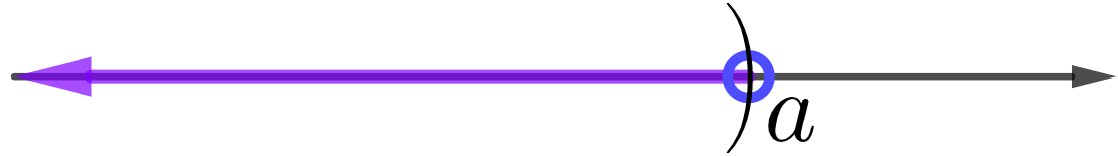
\includegraphics{figs/Interval-number-line-less-than.png} & 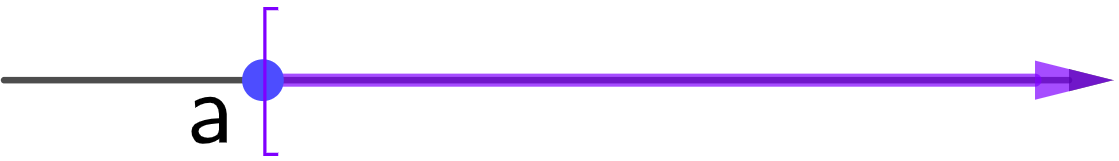
\includegraphics{figs/Interval-number-line-greater-than.png} & 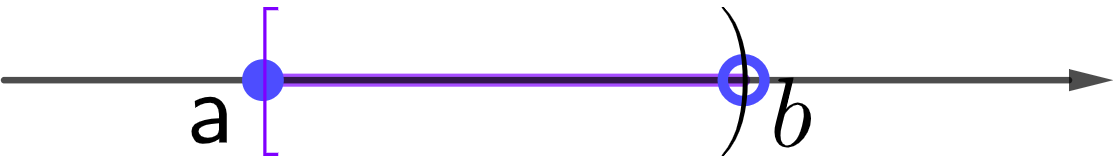
\includegraphics{figs/Interval-number-line-between.png} & 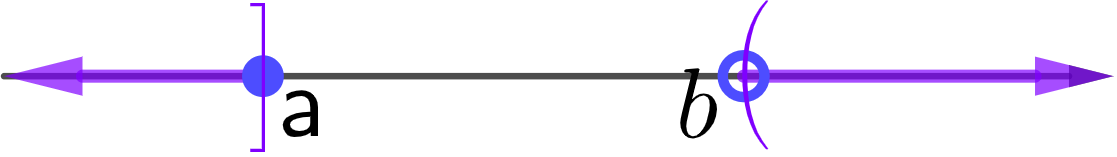
\includegraphics{figs/Interval-number-line-beyond.png}\tabularnewline
\((-\infty, a)\) & \([b,\infty)\) & \([a, b)\) & \((-\infty, a]\cup (b,\infty)\)\tabularnewline
\bottomrule
\end{longtable}

\hypertarget{examples-1}{%
\section{Examples}\label{examples-1}}

\BeginKnitrBlock{rmdtip}
\textbf{Think backward.} To solve a problem, knowing what to expect helps you narrow down the gap step by step by comparing the goal and your achievement.

An inequality (equation) is solved if the unknown variable is isolated. That's what to be expected. To isolate the unknown variable, you use comparisons to determine what mathematical operations should be applied. When an operation is applied to one side, the same operation should also be applied to the other side. For inequalities, we also need to determine whether the inequality sign should be preserved or reversed according to the operation.
\EndKnitrBlock{rmdtip}

\BeginKnitrBlock{example}
\protect\hypertarget{exm:unnamed-chunk-58}{}{\label{exm:unnamed-chunk-58} }Solve the linear inequality
\[
2x+4>0.
\]
\EndKnitrBlock{example}

\BeginKnitrBlock{solution}
\iffalse{} {Solution. } \fi{}\[
\begin{aligned}
&  & 2x+4 & >0  \\
    \text{add $-4$}      &  & 2x   & >-4 \\
    \text{divide by $2$} &  & x    & >-2
\end{aligned}
\]
The solution set is \((-2, \infty)\).
\EndKnitrBlock{solution}

\BeginKnitrBlock{example}
\protect\hypertarget{exm:unnamed-chunk-60}{}{\label{exm:unnamed-chunk-60} }Solve the linear inequality
\[
-3x-4<2.
\]
\EndKnitrBlock{example}

\BeginKnitrBlock{solution}
\iffalse{} {Solution. } \fi{}\[
\begin{aligned}
                                        &  & -3x-4 & <2       \\
    \text{add $4$}                   &  & -3x   & <6  &  & \\
    \text{divide by $-3$ and switch} &  & x     & >-2
\end{aligned}
\]
The solution set is \((-2, +\infty)\).
\EndKnitrBlock{solution}

\BeginKnitrBlock{example}
\protect\hypertarget{exm:unnamed-chunk-62}{}{\label{exm:unnamed-chunk-62} }Solve the compound linear inequality
\[
x+2<3\quad \text{and}\quad -2x-3<1.
\]
\EndKnitrBlock{example}

\BeginKnitrBlock{solution}
\iffalse{} {Solution. } \fi{}\[
\begin{aligned}
    x+2 & <3 &  & \text{and} & -2x-3 & <1  \\
    x   & <1 &  &            & -2x   & <4  \\
    x   & <1 &  & \text{and} & x     & >-2
\end{aligned}
\]
That is \(-2<x<1\). The solution set is \((-2, 1)\).
\EndKnitrBlock{solution}

\BeginKnitrBlock{example}
\protect\hypertarget{exm:unnamed-chunk-64}{}{\label{exm:unnamed-chunk-64} }Solve the compound linear inequality\\
\[
-x+4>2 \quad \text{or} \quad 2x-5\geq -3.
\]
\EndKnitrBlock{example}

\BeginKnitrBlock{solution}
\iffalse{} {Solution. } \fi{}\[
\begin{aligned}
    -x+4 & >2  &  & \text{or} & 2x-5 & \geq -3 \\
    -x   & >-2 &  &           & 2x   & \geq 2  \\
    x    & <2  &  & \text{or} & x    & \geq 1
\end{aligned}
\]
That is \(x\geq 1\) or \(x< 2\). The solution set is \((-\infty, +\infty)\).
\EndKnitrBlock{solution}

\BeginKnitrBlock{example}
\protect\hypertarget{exm:unnamed-chunk-66}{}{\label{exm:unnamed-chunk-66} }Solve the compound linear inequality
\[
-4\leq\dfrac{2x-4}{3}<2.
\]
\EndKnitrBlock{example}

\BeginKnitrBlock{solution}
\iffalse{} {Solution. } \fi{}\[
\begin{array}{rcl}
    -4\leq  & \dfrac{2x-4}{3}    & <2  \\
    -12\leq & 2x-4         & <6  \\
    -8\leq  & 2x                & <10 \\
    -4\leq  & x               & <5  
\end{array}
\]
The solution set is \([-4, 5)\).
\EndKnitrBlock{solution}

\BeginKnitrBlock{example}
\protect\hypertarget{exm:unnamed-chunk-68}{}{\label{exm:unnamed-chunk-68} }Solve the compound linear inequality
\[
-1\leq \dfrac{-3x+4}{2}<3.
\]
\EndKnitrBlock{example}

\BeginKnitrBlock{solution}
\iffalse{} {Solution. } \fi{}\[
\begin{array}{rcl}
    -1\leq & \frac{-3x+4}{2}  & <3        \\
    -2\leq & -3x+4          & <6        \\
    -6\leq & -3x           & <2        \\
    2\geq  & x            & >-\frac23
\end{array}
\]
The solution set is \((-\frac23, 2]\).
\EndKnitrBlock{solution}

\BeginKnitrBlock{example}
\protect\hypertarget{exm:unnamed-chunk-70}{}{\label{exm:unnamed-chunk-70} }
Suppose that \(-1\le x < 2\). Find the range of \(5-3x\). Write your answer in interval notation.
\EndKnitrBlock{example}

\BeginKnitrBlock{solution}
\iffalse{} {Solution. } \fi{}
To get \(5-3x\) from \(x\), we need first multiply \(x\) be \(-3\) and then add \(5\).
\[
\begin{array}{rcl}
-1\leq & x          & < 2        \\
3\geq & -3x         & >-6        \\
8\geq & 5-3x      & >-1
\end{array}
\]
The range of \(5-3x\) is \((-1, 8]\).
\EndKnitrBlock{solution}

\BeginKnitrBlock{rmdtip}
\textbf{Understand the Problem.} Understanding the known, the unknown and the condition of the given problem is the key to solve the problem. Normally, by comparing the known and unknown, you will find the way to solve the problem.
\EndKnitrBlock{rmdtip}

\hypertarget{practice-2}{%
\section{Practice}\label{practice-2}}

\BeginKnitrBlock{exercise}
\protect\hypertarget{exr:unnamed-chunk-73}{}{\label{exr:unnamed-chunk-73} }
Solve the linear inequality. \textbf{Write your answer in interval notation.}

\begin{enumerate}
\def\labelenumi{\arabic{enumi}.}
\tightlist
\item
  \(3x + 7 \leq 1\)
\item
  \(2x-3>1\)
\end{enumerate}
\EndKnitrBlock{exercise}

\BeginKnitrBlock{exercise}
\protect\hypertarget{exr:unnamed-chunk-74}{}{\label{exr:unnamed-chunk-74} }
Solve the linear inequality. \textbf{Write your answer in interval notation.}

\begin{enumerate}
\def\labelenumi{\arabic{enumi}.}
\tightlist
\item
  \(4x + 7 > 2x-3\)
\item
  \(3-2x \le x-6\)
\end{enumerate}
\EndKnitrBlock{exercise}

\BeginKnitrBlock{exercise}
\protect\hypertarget{exr:unnamed-chunk-75}{}{\label{exr:unnamed-chunk-75} }
Solve the compound linear inequality. \textbf{Write your answer in interval notation.}

\begin{enumerate}
\def\labelenumi{\arabic{enumi}.}
\tightlist
\item
  \(3x+2>-1 ~\text{and}~ 2x-7\leq 1\)
\item
  \(4x -7< 5 ~\text{and}~ 5x-2\geq 3\)
\end{enumerate}
\EndKnitrBlock{exercise}

\BeginKnitrBlock{exercise}
\protect\hypertarget{exr:unnamed-chunk-76}{}{\label{exr:unnamed-chunk-76} }
Solve the compound linear inequality. \textbf{Write your answer in interval notation.}

\begin{enumerate}
\def\labelenumi{\arabic{enumi}.}
\tightlist
\item
  \(-4\leq 3x+5<11\)
\item
  \(7\geq 2x-3\geq -7\)
\end{enumerate}
\EndKnitrBlock{exercise}

\BeginKnitrBlock{exercise}
\protect\hypertarget{exr:unnamed-chunk-77}{}{\label{exr:unnamed-chunk-77} }
Solve the compound linear inequality. \textbf{Write your answer in interval notation.}

\begin{enumerate}
\def\labelenumi{\arabic{enumi}.}
\tightlist
\item
  \(3x-5>-2 ~\text{or}~ 10-2x\leq 4\)
\item
  \(2x + 7<5 ~\text{or}~ 3x-8\geq x-2\)
\end{enumerate}
\EndKnitrBlock{exercise}

\BeginKnitrBlock{exercise}
\protect\hypertarget{exr:unnamed-chunk-78}{}{\label{exr:unnamed-chunk-78} }
Solve the compound linear inequality. \textbf{Write your answer in interval notation.}

\begin{enumerate}
\def\labelenumi{\arabic{enumi}.}
\tightlist
\item
  \(-2\leq \dfrac{2x-5}{3}<3\)
\item
  \(-1< \dfrac{3x+7}{2}\leq 4\)
\end{enumerate}
\EndKnitrBlock{exercise}

\BeginKnitrBlock{exercise}
\protect\hypertarget{exr:unnamed-chunk-79}{}{\label{exr:unnamed-chunk-79} }
Solve the linear inequality. \textbf{Write your answer in interval notation.}
\[
\frac13x+1<\frac12(2x-3)-1
\]
\EndKnitrBlock{exercise}

\BeginKnitrBlock{exercise}
\protect\hypertarget{exr:unnamed-chunk-80}{}{\label{exr:unnamed-chunk-80} }
Solve the compound linear inequality. \textbf{Write your answer in interval notation.}
\[
0\le \frac25-\frac{x+1}{3}< 1
\]
\EndKnitrBlock{exercise}

\BeginKnitrBlock{exercise}
\protect\hypertarget{exr:unnamed-chunk-81}{}{\label{exr:unnamed-chunk-81} }
Suppose \(0< x \le 1\). Find the range of \(-2x+1\). \textbf{Write your answer in interval notation.}
\EndKnitrBlock{exercise}

\BeginKnitrBlock{exercise}
\protect\hypertarget{exr:unnamed-chunk-82}{}{\label{exr:unnamed-chunk-82} }
Suppose that \(x+2y=1\) and \(1\leq x< 3\). Find the range of \(y\). \textbf{Write your answer in interval notation.}
\EndKnitrBlock{exercise}

\BeginKnitrBlock{exercise}
\protect\hypertarget{exr:unnamed-chunk-83}{}{\label{exr:unnamed-chunk-83} }
A toy store has a promotion ``Buy one get the second one half price'' on a certain popular toy. The sale price of the toy is \$20 each. Suppose the store makes more profit when you buy two. What do you think the store's purchasing price of the toy is?
\EndKnitrBlock{exercise}

\hypertarget{part-part-3-functions-and-applications}{%
\part*{Part 3: Functions and Applications}\label{part-part-3-functions-and-applications}}
\addcontentsline{toc}{part}{Part 3: Functions and Applications}

\hypertarget{introduction-to-functions}{%
\chapter{Introduction to Functions}\label{introduction-to-functions}}

\hypertarget{sets-order-pairs-and-the-rectangular-coordinate-system}{%
\section{Sets, Order Pairs, and the Rectangular Coordinate System}\label{sets-order-pairs-and-the-rectangular-coordinate-system}}

\hypertarget{functions-defined-by-equations}{%
\section{Functions Defined by Equations}\label{functions-defined-by-equations}}

\hypertarget{graphs-of-functions}{%
\section{Graphs of Functions}\label{graphs-of-functions}}

\hypertarget{linear-functions}{%
\chapter{Linear Functions}\label{linear-functions}}

\hypertarget{quadratic-functions}{%
\chapter{Quadratic Functions}\label{quadratic-functions}}

\hypertarget{the-complete-square-form}{%
\section{The Complete Square Form}\label{the-complete-square-form}}

\hypertarget{rational-and-radical-functions}{%
\chapter{Rational and Radical Functions}\label{rational-and-radical-functions}}

\hypertarget{exponential-functions}{%
\chapter{Exponential Functions}\label{exponential-functions}}

\hypertarget{logarithmic-functions}{%
\chapter{Logarithmic Functions}\label{logarithmic-functions}}

\hypertarget{applications-of-exponential-and-logarithmic-functions}{%
\chapter{Applications of Exponential and Logarithmic Functions}\label{applications-of-exponential-and-logarithmic-functions}}

\hypertarget{exponential-equations}{%
\section{Exponential Equations}\label{exponential-equations}}

\hypertarget{logarithmic-equations}{%
\section{Logarithmic Equations}\label{logarithmic-equations}}

\hypertarget{applications}{%
\section{Applications}\label{applications}}
% 参考文献


% 插入 after_body.tex

\end{document}
